\documentclass[11pt,a4paper]{article}

\usepackage[utf8]{inputenc}
\usepackage[T1]{fontenc}
\usepackage{mathpazo}
\usepackage[scaled=0.92]{helvet}
\usepackage[margin=1in]{geometry}
\usepackage{graphicx}
\usepackage{amsmath,amssymb,amsfonts}
\usepackage{booktabs}
\usepackage{tabularx}
\usepackage{setspace}
\usepackage{titlesec}
\usepackage{fancyhdr}
\usepackage{float}
\usepackage{caption}
\usepackage{microtype}
\usepackage{tikz}
\usepackage{xcolor}
\usepackage[hidelinks]{hyperref}

\usetikzlibrary{shapes.geometric, arrows.meta, positioning, calc, matrix, fit, backgrounds}

\setstretch{1.15}
\setlength{\parindent}{0pt}
\setlength{\parskip}{0.8em}
\sloppy

\titleformat{\section}{\normalfont\large\bfseries\sffamily}{\thesection}{1em}{}
\titleformat{\subsection}{\normalfont\normalsize\bfseries\sffamily}{\thesubsection}{1em}{}
\titleformat{\subsubsection}{\normalfont\normalsize\itshape\sffamily}{\thesubsubsection}{1em}{}

\pagestyle{fancy}
\fancyhf{}
\fancyhead[L]{\small\sffamily Atomik dan Kardinalitas dalam Basis Data}
\fancyhead[R]{\small\sffamily\thepage}
\renewcommand{\headrulewidth}{0.4pt}

\captionsetup{font=small,labelfont=bf,labelsep=period}

\renewenvironment{abstract}
{\small
	\begin{center}\textbf{\sffamily Abstrak}\end{center}
	\begin{quote}}
	{\end{quote}}

\lstdefinestyle{code}{
	basicstyle=\ttfamily\small,
	frame=single,
	rulecolor=\color{black},
	breaklines=true,
	showstringspaces=false,
	columns=fullflexible,
	keepspaces=true,
	framesep=6pt,
	aboveskip=1em,
	belowskip=1em,
	xleftmargin=0pt
}

\lstdefinestyle{out}{
	basicstyle=\ttfamily\small,
	frame=tb,
	rulecolor=\color{black},
	breaklines=true,
	showstringspaces=false,
	columns=fullflexible,
	keepspaces=true,
	framesep=4pt,
	aboveskip=1em,
	belowskip=1em
}

\title{\vspace{-1.5cm}\textbf{\sffamily\LARGE Atomik dan Kardinalitas\\ Dua Konsep Berbeda dalam Perancangan Basis Data Relasional}}
\author{
	\textbf{Muhammad Riduwan Khafidi} \\
	\small Program Studi Teknik Rekayasa Perangkat Lunak \\
	\small Politeknik Negeri Batam \\
	\small \texttt{4342611034@students.polibatam.ac.id}
}
\date{\small\today}

\begin{document}

\maketitle
\thispagestyle{empty}

\begin{abstract}
	Dua konsep yang sering tertukar dalam perancangan basis data relasional adalah atomik dan kardinalitas. Atomik berbicara tentang isi satu sel, sedangkan kardinalitas berbicara tentang aturan hubungan antar tabel. Makalah ini meluruskan kesalahpahaman yang lazim muncul: bahwa 1:1 berarti foreign key hanya ditulis satu kali, dan 1:N berarti foreign key boleh ditulis berkali-kali. Intuisi tersebut sebenarnya hampir benar, tetapi perlu diperjelas karena yang membatasi bukan jumlah penulisan, melainkan ada atau tidaknya constraint \texttt{UNIQUE} pada foreign key. Makalah ini menyajikan sepuluh visualisasi, mulai dari perbandingan atomik dan non-atomik, anatomi tiga jenis kardinalitas, hingga simulasi insert yang menunjukkan kapan constraint menolak data. Studi kasus sembilan langkah membangun skema dosen-mahasiswa dari nol melengkapi pembahasan.
\end{abstract}

\section{Pendahuluan}

\subsection{Analogi Pembuka: Loker Kantor dan Aturan Tamu}

Bayangkan sebuah kantor dengan dua hal yang perlu diatur. Pertama, loker karyawan. Setiap loker punya satu pintu, satu kunci, satu label nama. Seorang karyawan tidak boleh menaruh dua tas di satu loker, karena nanti tas kedua akan tertumpuk dan sulit diambil. Aturan "satu loker satu barang" inilah yang disebut atomik.

Kedua, aturan tamu. Ada perusahaan yang menerapkan aturan "satu direktur hanya boleh punya satu sekretaris pribadi". Ada perusahaan lain yang menerapkan "satu manajer boleh punya banyak staf, tetapi satu staf hanya dilayani satu manajer". Ada juga perusahaan konsultan yang menerapkan "banyak konsultan boleh mengerjakan banyak proyek, dan banyak proyek boleh dikerjakan banyak konsultan". Aturan "siapa boleh berpasangan dengan siapa" inilah yang disebut kardinalitas.

Dua hal ini berbeda. Loker adalah soal isi satu sel. Kardinalitas adalah soal hubungan antar tabel. Keduanya sering tertukar karena seorang pemula yang mencoba membuat relasi 1:N kadang menyelesaikannya dengan menaruh daftar nama di satu sel, yang justru melanggar atomik.

\subsection{Mengapa Topik Ini Penting}

Dalam ujian basis data, pertanyaan tentang kardinalitas hampir selalu muncul. Bentuknya bisa bermacam-macam: menentukan jenis relasi dari sebuah studi kasus, menggambar ERD, atau mengonversi ERD menjadi skema tabel. Kesalahan paling umum bukan pada menggambar, melainkan pada penempatan foreign key. Mahasiswa sering menaruh foreign key di sisi yang salah, atau lupa menambahkan \texttt{UNIQUE} ketika seharusnya 1:1, sehingga skema yang dihasilkan tidak sesuai dengan aturan bisnis yang diminta.

Selain itu, ada kesalahpahaman konseptual yang lebih dalam: mengira bahwa 1:1 berarti foreign key hanya ditulis sekali di dalam perintah \texttt{CREATE TABLE}, dan 1:N berarti boleh ditulis berkali-kali. Padahal dalam perintah \texttt{CREATE TABLE}, foreign key selalu ditulis sekali, terlepas dari kardinalitasnya. Yang berbeda adalah ada atau tidaknya constraint \texttt{UNIQUE} yang menemaninya.

\subsection{Peta Pembahasan}

Makalah ini dibagi menjadi empat bagian utama. Bagian kedua membahas atomik dan mengapa ia adalah fondasi yang tidak bisa ditawar. Bagian ketiga membahas kardinalitas dan meluruskan tiga kesalahpahaman umum. Bagian keempat menyajikan anatomi tiga jenis kardinalitas dengan simulasi insert yang menunjukkan kapan constraint menolak data. Bagian kelima menyandingkan ketiganya dalam satu tabel perbandingan. Bagian keenam membawa seluruh konsep ke studi kasus sembilan langkah membangun skema dosen-mahasiswa.

\section{Atomik: Fondasi yang Sering Terlupakan}

\subsection{Definisi Atomik}

Atomik berarti tidak dapat dibagi lagi. Dalam konteks basis data relasional, atomik berarti setiap sel dalam tabel hanya boleh berisi satu nilai dari tipe yang telah ditentukan. Bukan daftar, bukan objek, bukan array, bukan JSON bertumpuk. Satu sel berisi satu nama, atau satu angka, atau satu tanggal. Tidak lebih.

Aturan ini adalah syarat pertama dari Normal Form pertama (1NF). Tanpa atomik, seluruh operasi SQL menjadi tidak dapat diandalkan: pencarian menjadi lambat, pengurutan menjadi tidak mungkin, dan agregasi menjadi tidak akurat.

\subsection{Perbandingan Atomik dan Non-Atomik}

Gambar~\ref{fig:atomic} membandingkan dua tabel yang menyimpan data mahasiswa. Tabel kiri atomik, tabel kanan tidak.

\begin{figure}[H]
	\centering
	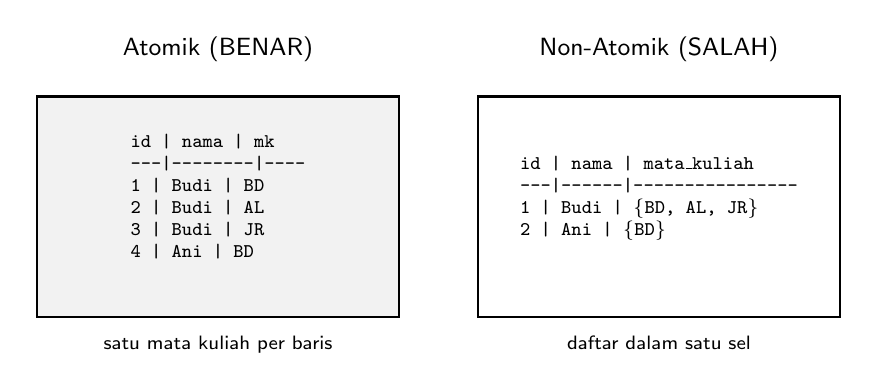
\begin{tikzpicture}[
			tbl/.style={rectangle, draw=black, thick, minimum width=4.6cm, minimum height=2.8cm, align=left, font=\ttfamily\scriptsize, inner sep=8pt},
			lbl/.style={font=\sffamily\small, align=center}
		]
		\node[lbl] at (-2.8, 2) {Atomik (BENAR)};
		\node[tbl, fill=black!5] (ok) at (-2.8, 0) {
			id | nama   | mk \\
			---|--------|---- \\
			1  | Budi   | BD \\
			2  | Budi   | AL \\
			3  | Budi   | JR \\
			4  | Ani    | BD \\
		};
		\node[font=\scriptsize\sffamily, below=0.1cm of ok, text width=4.6cm, align=center] {satu mata kuliah per baris};

		\node[lbl] at (2.8, 2) {Non-Atomik (SALAH)};
		\node[tbl, fill=white] (bad) at (2.8, 0) {
			id | nama | mata\_kuliah \\
			---|------|---------------- \\
			1  | Budi | \{BD, AL, JR\} \\
			2  | Ani  | \{BD\} \\
		};
		\node[font=\scriptsize\sffamily, below=0.1cm of bad, text width=4.6cm, align=center] {daftar dalam satu sel};
	\end{tikzpicture}
	\caption{Perbandingan tabel atomik dan non-atomik untuk data mahasiswa.}
	\label{fig:atomic}
\end{figure}

Tabel kanan menyimpan daftar di dalam satu sel. Ini terlihat hemat karena hanya ada dua baris, tetapi menimbulkan tiga masalah. Pertama, pencarian "siapa saja yang mengambil Algoritma" harus membaca seluruh sel, bukan sekadar mencocokkan nilai. Kedua, tidak mungkin menambahkan indeks pada sel yang berisi daftar. Ketiga, tidak ada cara mudah untuk menghapus satu mata kuliah tanpa menulis ulang seluruh sel.

\subsection{Mengapa Atomik Bukan Kardinalitas}

Ini titik yang paling sering membingungkan. Atomik dan kardinalitas terlihat mirip karena keduanya membatasi apa yang boleh masuk ke tabel, tetapi keduanya berada di level yang berbeda.

Gambar~\ref{fig:tree} memetakan posisi keduanya dalam perancangan basis data.

\begin{figure}[H]
	\centering
	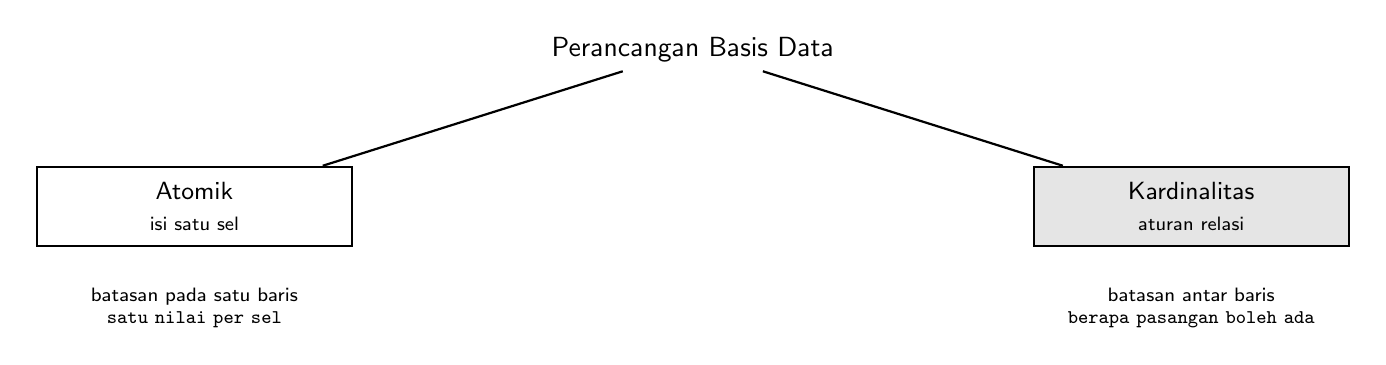
\begin{tikzpicture}[
			node distance=0.5cm and 0.8cm,
			cat/.style={rectangle, draw=black, thick, minimum width=4cm, minimum height=1cm, align=center, font=\sffamily\small},
			line/.style={draw, thick}
		]
		\node[font=\sffamily] (root) at (0, 1) {Perancangan Basis Data};
		\node[cat, fill=white, below left=1.2cm and 2.4cm of root] (atom) {Atomik \\ \scriptsize isi satu sel};
		\node[cat, fill=black!10, below right=1.2cm and 2.4cm of root] (card) {Kardinalitas \\ \scriptsize aturan relasi};

		\draw[line] (root) -- (atom);
		\draw[line] (root) -- (card);

		\node[font=\scriptsize\sffamily, below=0.4cm of atom, text width=4cm, align=center] {batasan pada satu baris \\ \texttt{satu nilai per sel}};
		\node[font=\scriptsize\sffamily, below=0.4cm of card, text width=4cm, align=center] {batasan antar baris \\ \texttt{berapa pasangan boleh ada}};
	\end{tikzpicture}
	\caption{Posisi atomik dan kardinalitas dalam perancangan basis data.}
	\label{fig:tree}
\end{figure}

Atomik adalah batasan pada level sel: satu sel satu nilai. Kardinalitas adalah batasan pada level relasi: berapa banyak baris dari tabel A boleh berpasangan dengan baris dari tabel B. Keduanya bisa dilanggar secara terpisah. Sebuah tabel bisa atomik tetapi kardinalitasnya salah (misalnya 1:1 yang seharusnya 1:N), atau sebaliknya.

Namun ada satu titik temu. Ketika seseorang mencoba membuat relasi 1:N tetapi tidak tahu caranya, ia sering menyelesaikannya dengan menaruh daftar nama mahasiswa di satu sel tabel dosen. Solusi ini melanggar atomik. Jadi pelanggaran atomik sering kali adalah gejala dari kesalahpahaman kardinalitas. Cara yang benar untuk membuat 1:N adalah dengan foreign key, bukan dengan daftar.

\section{Kardinalitas: Apa yang Sebenarnya Dibatasi}

\subsection{Definisi Kardinalitas}

Kardinalitas adalah aturan yang menentukan berapa banyak baris dari satu tabel boleh berpasangan dengan baris dari tabel lain. Ada tiga jenis yang perlu dikuasai, yaitu 1:1, 1:N, dan N:M.

Yang dibatasi oleh kardinalitas bukan primary key, karena primary key selalu unik di dalam tabelnya sendiri. Yang dibatasi adalah pasangan relasinya. Contohnya, dalam relasi dosen-mahasiswa, yang menjadi pertanyaan kardinalitas adalah: bolehkah satu dosen berpasangan dengan banyak mahasiswa, dan bolehkah satu mahasiswa berpasangan dengan banyak dosen.

\subsection{Meluruskan Tiga Miskonsepsi}

Miskonsepsi pertama, mengira 1:1 berarti foreign key hanya ditulis sekali di dalam perintah \texttt{CREATE TABLE}. Ini keliru. Dalam perintah \texttt{CREATE TABLE}, foreign key selalu ditulis sekali, terlepas dari kardinalitasnya. Yang membuat 1:1 menjadi 1:1 adalah tambahan constraint \texttt{UNIQUE} pada foreign key tersebut.

Miskonsepsi kedua, mengira 1:N berarti foreign key boleh ditulis berkali-kali di dalam perintah \texttt{CREATE TABLE}. Ini juga keliru. Yang membuat 1:N menjadi 1:N adalah tidak adanya constraint \texttt{UNIQUE}, bukan jumlah penulisan foreign key dalam perintah.

Miskonsepsi ketiga, mengira penempatan foreign key di 1:1 bebas di sisi mana saja tanpa syarat. Ini setengah benar. Foreign key memang boleh ditaruh di salah satu sisi, tetapi harus ditambah \texttt{UNIQUE} agar relasinya benar-benar 1:1. Tanpa \texttt{UNIQUE}, relasinya akan menjadi 1:N.

\subsection{Intuisi yang Benar}

Di balik tiga miskonsepsi tersebut, ada satu intuisi yang sebenarnya sudah benar: dalam 1:1, nilai foreign key hanya boleh muncul paling banyak satu kali di kolomnya; dalam 1:N, nilai foreign key boleh muncul berkali-kali. Gambar~\ref{fig:intuition} memvisualkan intuisi ini.

\begin{figure}[H]
	\centering
	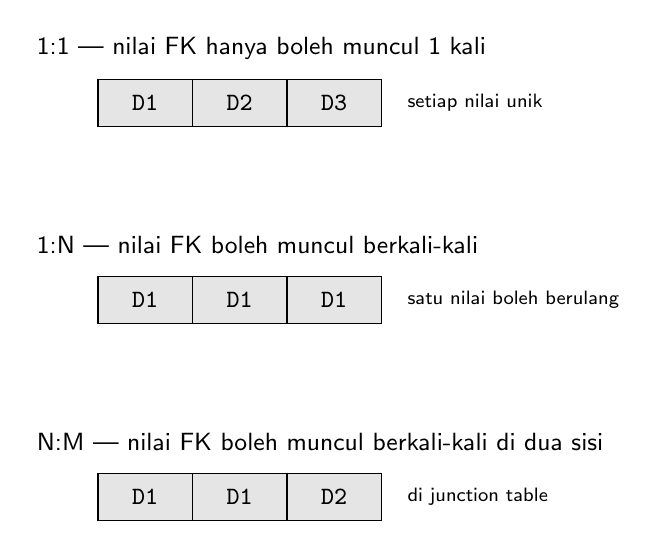
\begin{tikzpicture}[
			cell/.style={rectangle, draw=black, minimum width=1.2cm, minimum height=0.6cm, font=\ttfamily\small, align=center},
			lbl/.style={font=\sffamily\small, align=left}
		]
		\node[lbl, anchor=west] at (-5, 2) {1:1 — nilai FK hanya boleh muncul 1 kali};
		\node[cell, fill=black!10] (a1) at (-3.5, 1.3) {D1};
		\node[cell, fill=black!10] (a2) at (-2.3, 1.3) {D2};
		\node[cell, fill=black!10] (a3) at (-1.1, 1.3) {D3};
		\node[font=\scriptsize\sffamily, right=0.2cm of a3] {setiap nilai unik};

		\node[lbl, anchor=west] at (-5, -0.5) {1:N — nilai FK boleh muncul berkali-kali};
		\node[cell, fill=black!10] (b1) at (-3.5, -1.2) {D1};
		\node[cell, fill=black!10] (b2) at (-2.3, -1.2) {D1};
		\node[cell, fill=black!10] (b3) at (-1.1, -1.2) {D1};
		\node[font=\scriptsize\sffamily, right=0.2cm of b3] {satu nilai boleh berulang};

		\node[lbl, anchor=west] at (-5, -3) {N:M — nilai FK boleh muncul berkali-kali di dua sisi};
		\node[cell, fill=black!10] (c1) at (-3.5, -3.7) {D1};
		\node[cell, fill=black!10] (c2) at (-2.3, -3.7) {D1};
		\node[cell, fill=black!10] (c3) at (-1.1, -3.7) {D2};
		\node[font=\scriptsize\sffamily, right=0.2cm of c3] {di junction table};
	\end{tikzpicture}
	\caption{Intuisi yang benar tentang kemunculan nilai foreign key.}
	\label{fig:intuition}
\end{figure}

Yang perlu ditambahkan pada intuisi ini adalah bagaimana aturan tersebut ditegakkan. Untuk 1:1, penegaknya adalah \texttt{UNIQUE}. Untuk 1:N, penegaknya adalah ketiadaan \texttt{UNIQUE}. Untuk N:M, penegaknya adalah primary key komposit di junction table.

\section{Anatomi Tiga Jenis Kardinalitas}

\subsection{Relasi 1:1: Foreign Key dengan UNIQUE}

Relasi 1:1 berarti satu baris di tabel A berpasangan dengan paling banyak satu baris di tabel B, dan sebaliknya. Contoh paling sederhana adalah relasi mahasiswa dengan kartu tanda mahasiswa (KTM). Satu mahasiswa punya satu KTM, satu KTM hanya untuk satu mahasiswa.

Implementasinya memakai foreign key di salah satu tabel, ditambah constraint \texttt{UNIQUE}.

\begin{lstlisting}[style=code]
CREATE TABLE mahasiswa (
    id_mahasiswa INT PRIMARY KEY,
    nama VARCHAR(100) NOT NULL,
    id_ktm INT UNIQUE,
    FOREIGN KEY (id_ktm)
        REFERENCES ktm(id_ktm)
);
\end{lstlisting}

Kata kunci \texttt{UNIQUE} pada kolom \texttt{id\_ktm} inilah yang membuat relasinya menjadi 1:1. Tanpa \texttt{UNIQUE}, kolom tersebut bisa berisi nilai yang sama berkali-kali, dan relasinya menjadi 1:N. Gambar~\ref{fig:one-one} menunjukkan anatomi lengkapnya.

\begin{figure}[H]
	\centering
	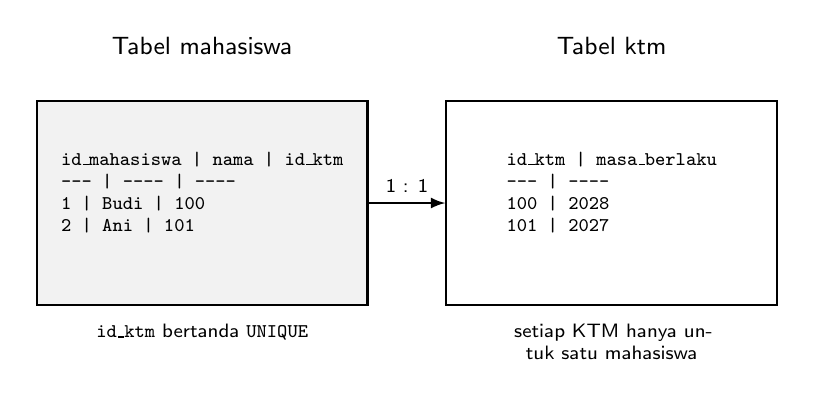
\begin{tikzpicture}[
			tbl/.style={rectangle, draw=black, thick, minimum width=4.2cm, minimum height=2.6cm, align=left, font=\ttfamily\scriptsize, inner sep=8pt},
			lbl/.style={font=\sffamily\small, align=center}
		]
		\node[lbl] at (-2.6, 2) {Tabel mahasiswa};
		\node[tbl, fill=black!5] (mhs) at (-2.6, 0) {
			id\_mahasiswa | nama | id\_ktm \\
			--- | ---- | ---- \\
			1 | Budi | 100 \\
			2 | Ani  | 101 \\
		};
		\node[font=\scriptsize\sffamily, below=0.1cm of mhs, text width=4.2cm, align=center] {\texttt{id\_ktm} bertanda \texttt{UNIQUE}};

		\node[lbl] at (2.6, 2) {Tabel ktm};
		\node[tbl, fill=white] (ktm) at (2.6, 0) {
			id\_ktm | masa\_berlaku \\
			--- | ---- \\
			100 | 2028 \\
			101 | 2027 \\
		};
		\node[font=\scriptsize\sffamily, below=0.1cm of ktm, text width=4.2cm, align=center] {setiap KTM hanya untuk satu mahasiswa};

		\draw[thick, -latex] (mhs) -- (ktm) node[midway, above, font=\scriptsize\sffamily] {1 : 1};
	\end{tikzpicture}
	\caption{Anatomi relasi 1:1 dengan foreign key ber-UNIQUE.}
	\label{fig:one-one}
\end{figure}

\subsection{Relasi 1:N: Foreign Key Tanpa UNIQUE}

Relasi 1:N berarti satu baris di tabel A boleh berpasangan dengan banyak baris di tabel B, tetapi satu baris di tabel B hanya berpasangan dengan satu baris di tabel A. Contohnya adalah relasi dosen dengan mahasiswa dalam konteks bimbingan akademik. Satu dosen membimbing banyak mahasiswa, tetapi satu mahasiswa hanya dibimbing satu dosen.

Implementasinya memakai foreign key di sisi N, yaitu di tabel mahasiswa, tanpa \texttt{UNIQUE}.

\begin{lstlisting}[style=code]
CREATE TABLE mahasiswa (
    id_mahasiswa INT PRIMARY KEY,
    nama VARCHAR(100) NOT NULL,
    id_dosen INT,
    FOREIGN KEY (id_dosen)
        REFERENCES dosen(id_dosen)
);
\end{lstlisting}

Perhatikan bahwa tidak ada \texttt{UNIQUE} pada kolom \texttt{id\_dosen}. Inilah yang memungkinkan satu dosen muncul berkali-kali di kolom tersebut, sesuai dengan relasi 1:N. Gambar~\ref{fig:one-n} menunjukkan anatomi lengkapnya.

\begin{figure}[H]
	\centering
	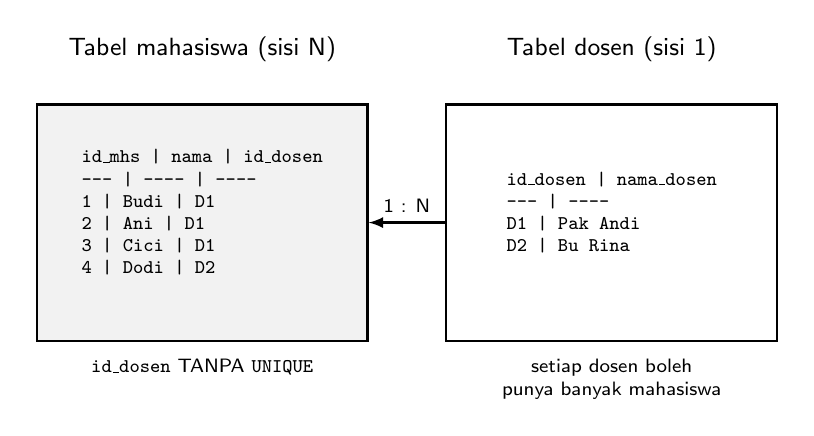
\begin{tikzpicture}[
			tbl/.style={rectangle, draw=black, thick, minimum width=4.2cm, minimum height=3cm, align=left, font=\ttfamily\scriptsize, inner sep=8pt},
			lbl/.style={font=\sffamily\small, align=center}
		]
		\node[lbl] at (-2.6, 2.2) {Tabel mahasiswa (sisi N)};
		\node[tbl, fill=black!5] (mhs) at (-2.6, 0) {
			id\_mhs | nama | id\_dosen \\
			--- | ---- | ---- \\
			1 | Budi | D1 \\
			2 | Ani  | D1 \\
			3 | Cici | D1 \\
			4 | Dodi | D2 \\
		};
		\node[font=\scriptsize\sffamily, below=0.1cm of mhs, text width=4.2cm, align=center] {\texttt{id\_dosen} TANPA \texttt{UNIQUE}};

		\node[lbl] at (2.6, 2.2) {Tabel dosen (sisi 1)};
		\node[tbl, fill=white] (dsn) at (2.6, 0) {
			id\_dosen | nama\_dosen \\
			--- | ---- \\
			D1 | Pak Andi \\
			D2 | Bu Rina \\
		};
		\node[font=\scriptsize\sffamily, below=0.1cm of dsn, text width=4.2cm, align=center] {setiap dosen boleh punya banyak mahasiswa};

		\draw[thick, -latex] (dsn) -- (mhs) node[midway, above, font=\scriptsize\sffamily] {1 : N};
	\end{tikzpicture}
	\caption{Anatomi relasi 1:N dengan foreign key di sisi N tanpa UNIQUE.}
	\label{fig:one-n}
\end{figure}

Nilai D1 muncul tiga kali di kolom \texttt{id\_dosen}, dan itu sah. Jika constraint \texttt{UNIQUE} ditambahkan, insert kedua akan ditolak, dan relasinya berubah menjadi 1:1.

\subsection{Relasi N:M: Tabel Penghubung}

Relasi N:M berarti banyak baris di tabel A boleh berpasangan dengan banyak baris di tabel B, dan sebaliknya. Contohnya adalah relasi mahasiswa dengan mata kuliah. Satu mahasiswa mengambil banyak mata kuliah, satu mata kuliah diambil banyak mahasiswa.

Relasi ini tidak bisa diimplementasikan dengan foreign key di salah satu tabel, karena foreign key hanya bisa menampung satu nilai per baris. Solusinya adalah junction table, yaitu tabel baru yang berisi dua foreign key dan primary key komposit.

\begin{lstlisting}[style=code]
CREATE TABLE krs (
    id_mahasiswa INT,
    id_mk INT,
    semester INT,
    PRIMARY KEY (id_mahasiswa, id_mk),
    FOREIGN KEY (id_mahasiswa)
        REFERENCES mahasiswa(id_mahasiswa),
    FOREIGN KEY (id_mk)
        REFERENCES mata_kuliah(id_mk)
);
\end{lstlisting}

Primary key komposit \texttt{(id\_mahasiswa, id\_mk)} mencegah pasangan yang sama muncul dua kali. Gambar~\ref{fig:n-m} menunjukkan tiga tabel yang terhubung.

\begin{figure}[H]
	\centering
	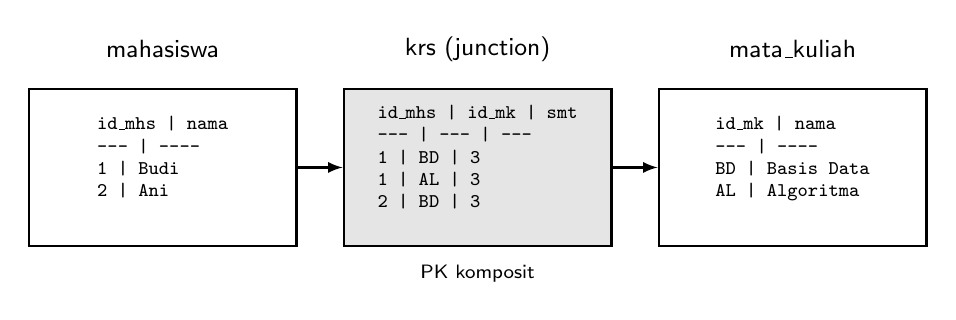
\begin{tikzpicture}[
			tbl/.style={rectangle, draw=black, thick, minimum width=3.4cm, minimum height=2cm, align=left, font=\ttfamily\scriptsize, inner sep=6pt},
			lbl/.style={font=\sffamily\small, align=center},
			line/.style={draw, thick, -latex}
		]
		\node[lbl] at (-4, 1.5) {mahasiswa};
		\node[tbl, fill=white] (m) at (-4, 0) {
			id\_mhs | nama \\
			--- | ---- \\
			1 | Budi \\
			2 | Ani \\
		};

		\node[lbl] at (0, 1.5) {krs (junction)};
		\node[tbl, fill=black!10] (k) at (0, 0) {
			id\_mhs | id\_mk | smt \\
			--- | --- | --- \\
			1 | BD | 3 \\
			1 | AL | 3 \\
			2 | BD | 3 \\
		};

		\node[lbl] at (4, 1.5) {mata\_kuliah};
		\node[tbl, fill=white] (mk) at (4, 0) {
			id\_mk | nama \\
			--- | ---- \\
			BD | Basis Data \\
			AL | Algoritma \\
		};

		\draw[line] (m) -- (k);
		\draw[line] (k) -- (mk);

		\node[font=\scriptsize\sffamily, below=0.1cm of k, text width=3.4cm, align=center] {PK komposit};
	\end{tikzpicture}
	\caption{Relasi N:M melalui junction table dengan PK komposit.}
	\label{fig:n-m}
\end{figure}

\subsection{Simulasi Insert: Kapan Constraint Menolak}

Untuk melihat langsung bagaimana constraint bekerja, mari simulasikan insert ke tiga skenario. Gambar~\ref{fig:simul} menampilkan hasilnya.

\begin{figure}[H]
	\centering
	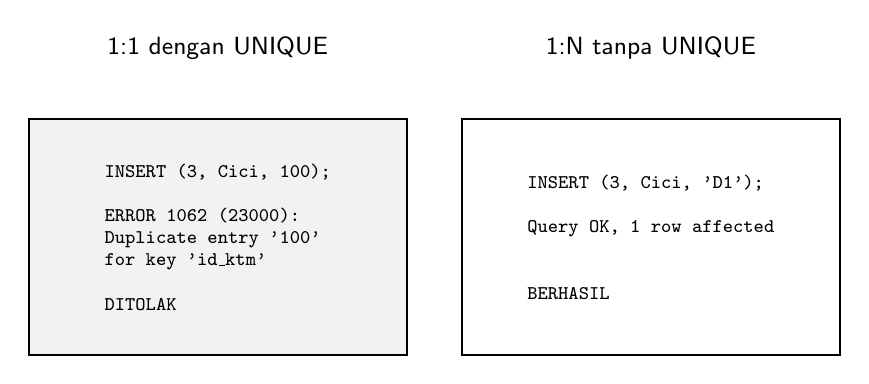
\begin{tikzpicture}[
			box/.style={rectangle, draw=black, thick, minimum width=4.8cm, minimum height=3cm, align=left, font=\ttfamily\scriptsize, inner sep=6pt},
			lbl/.style={font=\sffamily\small, align=center}
		]
		\node[lbl] at (-3, 2.4) {1:1 dengan UNIQUE};
		\node[box, fill=black!5] (one) at (-3, 0) {
			INSERT (3, Cici, 100); \\
			\ \\
			ERROR 1062 (23000): \\
			Duplicate entry '100' \\
			for key 'id\_ktm' \\
			\ \\
			DITOLAK
		};

		\node[lbl] at (2.5, 2.4) {1:N tanpa UNIQUE};
		\node[box, fill=white] (many) at (2.5, 0) {
			INSERT (3, Cici, 'D1'); \\
			\ \\
			Query OK, 1 row affected \\
			\ \\
			\ \\
			BERHASIL
		};
	\end{tikzpicture}
	\caption{Simulasi insert: UNIQUE menolak duplikasi, tanpa UNIQUE mengizinkan.}
	\label{fig:simul}
\end{figure}

Perhatikan dua hal. Pertama, insert ke skema 1:1 dengan nilai \texttt{id\_ktm} yang sudah ada akan ditolak dengan pesan \texttt{Duplicate entry}. Kedua, insert ke skema 1:N dengan nilai \texttt{id\_dosen} yang sudah ada akan berhasil. Inilah bukti bahwa \texttt{UNIQUE} adalah penegak kardinalitas 1:1.

\section{Perbandingan Lintas Kardinalitas}

Tabel~\ref{tab:comparison} menyandingkan tiga jenis kardinalitas pada delapan aspek.

\begin{table}[H]
	\centering
	\caption{Perbandingan tiga jenis kardinalitas.}
	\label{tab:comparison}
	\footnotesize
	\begin{tabularx}{\textwidth}{l X X X}
		\toprule
		Aspek & 1:1 & 1:N & N:M \\
		\midrule
		Definisi & satu berpasangan satu & satu berpasangan banyak & banyak berpasangan banyak \\
		Contoh & mahasiswa dan KTM & dosen dan mahasiswa & mahasiswa dan mata kuliah \\
		Penempatan FK & salah satu sisi & sisi N & junction table \\
		Constraint kunci & \texttt{UNIQUE} & tanpa \texttt{UNIQUE} & PK komposit \\
		Kemunculan FK & paling banyak sekali & berkali-kali & berkali-kali di dua sisi \\
		Bentuk tabel tambahan & tidak perlu & tidak perlu & wajib junction \\
		Kesalahan lazim & lupa \texttt{UNIQUE} & FK di sisi yang salah & tidak buat junction \\
		Insert kedua dengan FK sama & ditolak & diterima & lihat PK komposit \\
		\bottomrule
	\end{tabularx}
\end{table}

Dua paragraf penutup dari perbandingan ini. Pertama, perbedaan 1:1 dan 1:N terletak pada satu kata kunci saja, yaitu \texttt{UNIQUE}. Kedua, perbedaan 1:N dan N:M terletak pada keberadaan tabel ketiga. Keduanya adalah perbedaan struktural yang bisa langsung dibaca dari perintah \texttt{CREATE TABLE}, bukan dari jumlah penulisan dalam perintah.

\section{Studi Kasus: Membangun Skema dari Nol}

Mari ikuti sembilan langkah membangun skema dosen-mahasiswa dari nol, dengan setiap keputusan dijelaskan.

\subsection{Langkah 1: Tentukan Kebutuhan}

Sebuah kampus membutuhkan skema untuk mencatat dosen, mahasiswa, dan bimbingan akademik. Satu dosen membimbing banyak mahasiswa, satu mahasiswa hanya dibimbing satu dosen.

\subsection{Langkah 2: Identifikasi Kardinalitas}

Dari kebutuhan tersebut, relasi antara dosen dan mahasiswa adalah 1:N. Sisi 1 adalah dosen, sisi N adalah mahasiswa.

\subsection{Langkah 3: Buat Tabel Dosen}

\begin{lstlisting}[style=code]
CREATE TABLE dosen (
    id_dosen INT PRIMARY KEY,
    nama_dosen VARCHAR(100) NOT NULL
);
\end{lstlisting}

\begin{lstlisting}[style=out]
Query OK, 0 rows affected
\end{lstlisting}

\subsection{Langkah 4: Buat Tabel Mahasiswa dengan Foreign Key di Sisi N}

\begin{lstlisting}[style=code]
CREATE TABLE mahasiswa (
    id_mahasiswa INT PRIMARY KEY,
    nama VARCHAR(100) NOT NULL,
    id_dosen INT,
    FOREIGN KEY (id_dosen)
        REFERENCES dosen(id_dosen)
);
\end{lstlisting}

Foreign key ditaruh di tabel \texttt{mahasiswa} karena itu adalah sisi N. Tidak ada \texttt{UNIQUE} karena relasinya 1:N.

\subsection{Langkah 5: Insert Data Uji}

\begin{lstlisting}[style=code]
INSERT INTO dosen VALUES (1, 'Pak Andi');
INSERT INTO dosen VALUES (2, 'Bu Rina');
INSERT INTO mahasiswa VALUES (1, 'Budi', 1);
INSERT INTO mahasiswa VALUES (2, 'Ani',  1);
INSERT INTO mahasiswa VALUES (3, 'Cici', 1);
\end{lstlisting}

\subsection{Langkah 6: Verifikasi Relasi 1:N}

\begin{lstlisting}[style=code]
SELECT * FROM mahasiswa WHERE id_dosen = 1;
\end{lstlisting}

\begin{lstlisting}[style=out]
+--------------+------+----------+
| id_mahasiswa | nama | id_dosen |
+--------------+------+----------+
|            1 | Budi |        1 |
|            2 | Ani  |        1 |
|            3 | Cici |        1 |
+--------------+------+----------+
3 rows in set
\end{lstlisting}

Tiga baris dengan \texttt{id\_dosen} sama membuktikan bahwa relasinya 1:N.

\subsection{Langkah 7: Ubah Menjadi 1:1}

Jika aturan kampus berubah menjadi "satu dosen hanya membimbing satu mahasiswa", tambahkan \texttt{UNIQUE}.

\begin{lstlisting}[style=code]
ALTER TABLE mahasiswa
    ADD UNIQUE (id_dosen);
\end{lstlisting}

Perintah ini akan gagal jika sudah ada lebih dari satu baris dengan \texttt{id\_dosen} yang sama. Pada data di atas, ada tiga baris dengan \texttt{id\_dosen} = 1, sehingga perintah ini akan ditolak.

\begin{lstlisting}[style=out]
ERROR 1062 (23000): Duplicate entry '1' for key 'id_dosen'
\end{lstlisting}

Ini membuktikan bahwa \texttt{UNIQUE} adalah penegak kardinalitas 1:1.

\subsection{Langkah 8: Ubah Menjadi N:M}

Jika aturan berubah menjadi "banyak dosen membimbing banyak mahasiswa", tidak ada cara untuk menyelesaikannya dengan satu foreign key. Perlu junction table.

\begin{lstlisting}[style=code]
CREATE TABLE bimbingan (
    id_dosen INT,
    id_mahasiswa INT,
    PRIMARY KEY (id_dosen, id_mahasiswa),
    FOREIGN KEY (id_dosen)
        REFERENCES dosen(id_dosen),
    FOREIGN KEY (id_mahasiswa)
        REFERENCES mahasiswa(id_mahasiswa)
);
\end{lstlisting}

\subsection{Langkah 9: Verifikasi Junction}

\begin{lstlisting}[style=code]
INSERT INTO bimbingan VALUES (1, 1);
INSERT INTO bimbingan VALUES (1, 2);
INSERT INTO bimbingan VALUES (2, 1);
\end{lstlisting}

\begin{lstlisting}[style=out]
+----------+--------------+
| id_dosen | id_mahasiswa |
+----------+--------------+
|        1 |            1 |
|        1 |            2 |
|        2 |            1 |
+----------+--------------+
3 rows in set
\end{lstlisting}

Dosen 1 membimbing mahasiswa 1 dan 2, dan mahasiswa 1 dibimbing dosen 1 dan 2. Ini adalah relasi N:M yang benar.

\subsection{Timeline Studi Kasus}

Gambar~\ref{fig:timeline} merangkum sembilan langkah dalam satu garis waktu.

\begin{figure}[H]
	\centering
	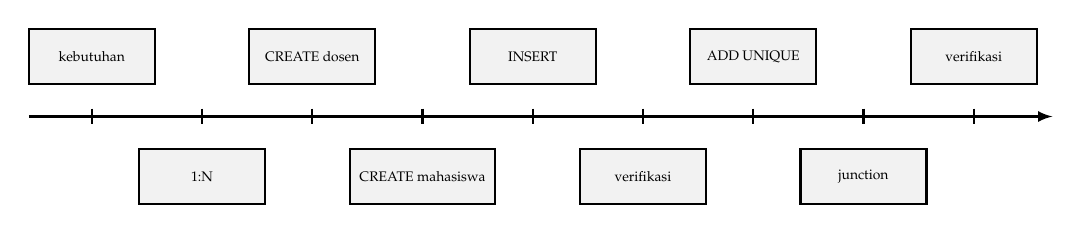
\begin{tikzpicture}[
			ev/.style={rectangle, draw=black, thick, fill=black!5, minimum width=1.6cm, minimum height=0.7cm, align=center, font=\tiny},
			line/.style={draw, thick}
		]
		\draw[line, -latex] (-6.5, 0) -- (6.5, 0);

		\draw[thick] (-5.7, 0.1) -- (-5.7, -0.1);
		\node[ev, above=0.2cm] at (-5.7, 0.2) {kebutuhan};

		\draw[thick] (-4.3, 0.1) -- (-4.3, -0.1);
		\node[ev, below=0.2cm] at (-4.3, -0.2) {1:N};

		\draw[thick] (-2.9, 0.1) -- (-2.9, -0.1);
		\node[ev, above=0.2cm] at (-2.9, 0.2) {CREATE dosen};

		\draw[thick] (-1.5, 0.1) -- (-1.5, -0.1);
		\node[ev, below=0.2cm] at (-1.5, -0.2) {CREATE mahasiswa};

		\draw[thick] (-0.1, 0.1) -- (-0.1, -0.1);
		\node[ev, above=0.2cm] at (-0.1, 0.2) {INSERT};

		\draw[thick] (1.3, 0.1) -- (1.3, -0.1);
		\node[ev, below=0.2cm] at (1.3, -0.2) {verifikasi};

		\draw[thick] (2.7, 0.1) -- (2.7, -0.1);
		\node[ev, above=0.2cm] at (2.7, 0.2) {ADD UNIQUE};

		\draw[thick] (4.1, 0.1) -- (4.1, -0.1);
		\node[ev, below=0.2cm] at (4.1, -0.2) {junction};

		\draw[thick] (5.5, 0.1) -- (5.5, -0.1);
		\node[ev, above=0.2cm] at (5.5, 0.2) {verifikasi};
	\end{tikzpicture}
	\caption{Timeline sembilan langkah studi kasus.}
	\label{fig:timeline}
\end{figure}

\section{Kesalahan Umum dan Cara Menghindarinya}

\begin{table}[H]
	\centering
	\caption{Kesalahan umum pada kardinalitas dan atomik.}
	\label{tab:mistakes}
	\footnotesize
	\begin{tabularx}{\textwidth}{l X X}
		\toprule
		Kesalahan & Akibat & Perbaikan \\
		\midrule
		daftar nama di satu sel & melanggar atomik & pecah jadi baris, pakai FK \\
		foreign key di sisi yang salah pada 1:N & relasi jadi 1:1 atau rusak & taruh di sisi N \\
		lupa \texttt{UNIQUE} pada 1:1 & relasi jadi 1:N & tambah \texttt{UNIQUE} pada FK \\
		tambah \texttt{UNIQUE} pada 1:N & relasi jadi 1:1 & hapus \texttt{UNIQUE} \\
		N:M tanpa junction & tidak bisa diimplementasikan & buat junction table \\
		junction tanpa PK komposit & duplikat pasangan & tambah \texttt{PRIMARY KEY (a,b)} \\
		\texttt{id\_dosen} sebagai PK di mahasiswa & satu mahasiswa hanya satu, PK-nya salah & gunakan PK sendiri \\
		\texttt{id\_mk} disimpan sebagai teks di mahasiswa & melanggar atomik & pakai junction table \\
		mengira \texttt{UNIQUE} sama dengan \texttt{PRIMARY KEY} & \texttt{UNIQUE} boleh NULL & PK tidak boleh NULL \\
		\texttt{ON DELETE} tanpa aksi & FK orphan & pakai \texttt{ON DELETE CASCADE} atau \texttt{RESTRICT} \\
		\bottomrule
	\end{tabularx}
\end{table}

Dua kesalahan yang paling sering muncul saat ujian adalah lupa \texttt{UNIQUE} pada 1:1 dan menaruh foreign key di sisi yang salah pada 1:N. Keduanya bisa dideteksi dengan satu pertanyaan sederhana: setelah insert data uji, apakah nilai foreign key boleh berulang? Jika boleh, maka 1:N. Jika tidak, maka 1:1 dengan \texttt{UNIQUE}.

\section{Lembar Rujukan Cepat}

\begin{table}[H]
	\centering
	\caption{Rujukan cepat kardinalitas dan atomik.}
	\label{tab:cheat}
	\footnotesize
	\begin{tabularx}{\textwidth}{l X}
		\toprule
		Kebutuhan & Solusi \\
		\midrule
		satu sel satu nilai & atomik, tidak ada daftar \\
		relasi 1:1 & FK di salah satu sisi + \texttt{UNIQUE} \\
		relasi 1:N & FK di sisi N, tanpa \texttt{UNIQUE} \\
		relasi N:M & junction table + PK komposit \\
		relasi 1:1 dengan FK sebagai PK & PK/FK combo, otomatis \texttt{UNIQUE} \\
		relasi opsional 1:1 & FK \texttt{NULL} + \texttt{UNIQUE} \\
		relasi wajib 1:1 & FK \texttt{NOT NULL} + \texttt{UNIQUE} \\
		relasi wajib 1:N & FK \texttt{NOT NULL} \\
		relasi opsional 1:N & FK \texttt{NULL} \\
		multi-nilai per baris & pecah ke tabel terpisah \\
		aturan bisnis "hanya satu" & \texttt{UNIQUE} \\
		aturan bisnis "boleh banyak" & tanpa \texttt{UNIQUE} \\
		verifikasi 1:N & cek apakah FK berulang di data uji \\
		verifikasi 1:1 & coba insert kedua dengan FK sama \\
		hapus anak saat induk dihapus & \texttt{ON DELETE CASCADE} \\
		tolak hapus induk jika ada anak & \texttt{ON DELETE RESTRICT} \\
		nilai FK jadi NULL saat induk dihapus & \texttt{ON DELETE SET NULL} \\
		cek constraint yang ada & \texttt{SHOW CREATE TABLE} \\
		cek index pada FK & \texttt{SHOW INDEX FROM tabel} \\
		lihat foreign key & \texttt{SELECT * FROM information\_schema.KEY\_COLUMN\_USAGE} \\
		\bottomrule
	\end{tabularx}
\end{table}

\section{Kesimpulan}

Atomik dan kardinalitas adalah dua konsep yang berbeda. Atomik berbicara tentang isi satu sel, sedangkan kardinalitas berbicara tentang aturan hubungan antar tabel. Pelanggaran atomik sering kali adalah gejala dari kesalahpahaman kardinalitas, seperti ketika seseorang mencoba membuat relasi 1:N dengan menaruh daftar nama di satu sel.

Intuisi bahwa 1:1 berarti nilai foreign key hanya boleh muncul sekali, dan 1:N berarti nilai foreign key boleh muncul berkali-kali, sebenarnya sudah benar. Yang perlu ditambahkan adalah mekanisme penegaknya: \texttt{UNIQUE} untuk 1:1, ketiadaan \texttt{UNIQUE} untuk 1:N, dan primary key komposit untuk N:M. Ketiganya adalah perbedaan struktural yang bisa dibaca langsung dari perintah \texttt{CREATE TABLE}, bukan dari jumlah penulisan foreign key dalam perintah tersebut.

Tiga prinsip penutup:

\begin{enumerate}
	\item Atomik dulu, baru kardinalitas. Pastikan setiap sel berisi satu nilai sebelum memikirkan relasi antar tabel. Daftar di dalam sel selalu salah, bukan hanya kurang rapi.
	\item \texttt{UNIQUE} adalah pembeda 1:1 dan 1:N. Tanpa \texttt{UNIQUE}, foreign key apa pun akan berperilaku 1:N. Menambahkan \texttt{UNIQUE} adalah satu-satunya cara membuatnya menjadi 1:1.
	\item N:M butuh tabel ketiga. Tidak ada jalan pintas. Junction table dengan primary key komposit adalah satu-satunya solusi yang benar, dan solusi ini sekaligus mencegah duplikat pasangan tanpa perlu trigger tambahan.
\end{enumerate}

Dengan kerangka mental ini, pertanyaan ujian berbentuk "tentukan kardinalitas" atau "konversi ERD menjadi tabel" dapat dijawab dengan alasan yang bisa dipertanggungjawabkan, bukan dengan hafalan.

\newpage
\section*{Referensi}
\addcontentsline{toc}{section}{Referensi}

\begin{thebibliography}{99}

	\bibitem{silberschatz}
	Silberschatz, A., Korth, H. F., \& Sudarshan, S. (2019).
	\textit{Database System Concepts} (7th ed.).
	McGraw-Hill Education.

	\bibitem{date}
	Date, C. J. (2003).
	\textit{An Introduction to Database Systems} (8th ed.).
	Addison-Wesley.

	\bibitem{elmasri}
	Elmasri, R., \& Navathe, S. B. (2016).
	\textit{Fundamentals of Database Systems} (7th ed.).
	Pearson.

	\bibitem{kleppmann}
	Kleppmann, M. (2017).
	\textit{Designing Data-Intensive Applications}.
	O'Reilly Media.

	\bibitem{codd}
	Codd, E. F. (1970).
	A Relational Model of Data for Large Shared Data Banks.
	\textit{Communications of the ACM}, 13(6), 377--387.

	\bibitem{mariadb-ddl}
	MariaDB Foundation. (2026).
	\textit{SQL Statements --- CREATE TABLE, ALTER TABLE, DROP TABLE}.
	MariaDB Knowledge Base.
	\texttt{https://mariadb.com/kb/en/sql-statements/}

	\bibitem{mysql-ddl}
	Oracle Corporation. (2026).
	\textit{MySQL 8.0 Reference Manual --- Data Definition Statements}.
	\texttt{https://dev.mysql.com/doc/refman/8.0/en/sql-data-definition-statements.html}

	\bibitem{postgresql}
	The PostgreSQL Global Development Group. (2026).
	\textit{SQL Commands --- CREATE TABLE, ALTER TABLE}.
	\texttt{https://www.postgresql.org/docs/current/sql-commands.html}

\end{thebibliography}

\end{document}